\begin{problem}{1} $ $

	\begin{enumerate}
		\item The characteristic polynomial for this recursive formula is
		
		\begin{equation*}
		x^2-2x+\frac{3}{4}=0,
		\end{equation*}
		which has roots 1/2 and 3/2, and therefore:		
		\begin{equation*}
		a_n=\alpha \left(\frac{3}{2} \right)^n+\beta \left(\frac{1}{2} \right)^n.
		\end{equation*}
		Using the initial conditions $a_0=1$ and $a_1=-1$ leads to $\alpha=-1$ and $\beta=1$.  Thus, the solution to the recurrence equation is:
		\begin{equation*}
		a_n=-\left(\frac{3}{2} \right)^n+ \left(\frac{1}{2} \right)^n.
		\end{equation*}
		
		\item  The characteristic polynomial for this recursive formula is
		
		\begin{equation*}
		x^2-4x+4=0,
		\end{equation*}
		which can be factored into $(x-2)^2=0$.  The polynomial thus has one root, $x=2$, with a multiplicity of 2, and therefore:
		\begin{equation*}
		a_n=\alpha 2^n+\beta n 2^n.
		\end{equation*}
		Using the initial conditions $a_0=2$ and $a_1=6$ leads to $\alpha=2$ and $\beta=1$.  Thus, the solution to the recurrence equation is:
		\begin{equation*}
		a_n=2n^{n+1}+n2^n.
		\end{equation*}

	\end{enumerate}

\end{problem}


\begin{problem}{2} $ $

	\begin{enumerate}
		\item Let $A_{n,k}$ be the event of observing exactly $k$ heads out of $n$ coin tosses, and let $H$ denote the event that the last coin toss is a heads.  By conditioning on the last coin toss I obtain:
		\begin{align*}
		P(A_{n, k}) &= P(A_{n, k}|H)p+P(A_{n, k}|H^c)(1-p) \\
		&= P(A_{n-1, k-1})p+P(A_{n-1, k})(1-p),
		\end{align*}
where the equality follows because if the last coin toss is heads, then we need exactly $k-1$ heads from the first $n-1$ tosses, and if the last coin toss is tails, then we need exactly $k$ heads from the first $n-1$ tosses.  Converting this to the notation used in the problem:
		\begin{equation*}
		a_{n,k}= a_{n-1, k-1}p+a_{n-1, k}(1-p)
		\end{equation*}
$\implies$
		\begin{equation*}
		a_{n+1,k+1}= a_{n, k}p+a_{n, k+1}(1-p).
		\end{equation*}

\item We recognize that this is precisely a binomial experiment, so the probability associated with exactly $k$ heads out of $n$ is given by $\binom{n}{k} p^k (1-p)^{n-k}$, and therefore, using the equation above,
		\begin{equation*}
		\binom{n+1}{k+1} p^{k+1} (1-p)^{(n+1)-(k+1)}= p\binom{n}{k} p^k (1-p)^{n-k}+(1-p)\binom{n}{k+1} p^{k+1} (1-p)^{n-(k+1)},
		\end{equation*}
which, when simplified results in:
		\begin{equation*}
		\binom{n+1}{k+1}= \binom{n}{k}+\binom{n}{k+1}.
		\end{equation*}
We need the restriction that $0 \le k <n$ to hold for this equation to be true, since the original recursion relation does not hold if $k = n$ (in that case the last flip cannot be a tails since we need all flips to be heads, so that the $P(A_{n, k}|H^c)$ term should be 0).
\end{enumerate}
\end{problem}

\begin{problem}{3} Let $A$ be the desired event and let $q=1-p$ be the probability of tails.  To solve this problem, I first condition on whether the first toss is a heads or tails:
\begin{equation*}
P(A) = P(A|H)p+P(A|T)q.
\end{equation*}
To help solve for $P(A|H)$, I now condition on the second toss:
\begin{align*}
P(A|H) &= P(A|HH)p+P(A|HT)q \\
&= 1\cdot p+P(A|T)q,
\end{align*}
where $P(A|HH) =1$ since if you flip 2 consecutive heads, the experiment is done and where $P(A|HT) = P(A|T)$, since the first heads does not matter because we are interested in 2 consecutive heads, and 1 isolated heads does not get us any closer to the event $A$.

To help solve for $P(A|T)$, I also condition on the second toss:
\begin{align*}
P(A|T) &= P(A|TH)p+P(A|TT)q \\
&= P(A|H)p +0\cdot q,
\end{align*}
where $P(A|TT) =0$ since if you flip 2 consecutive tails, the experiment is done (and the desired even did not occur) and where $P(A|TH) = P(A|H)$, for essentially the same reason that $P(A|HT) = P(A|T)$ as described above.

I now re-express these 3 equations in slightly more readable notation:
 \[
\left\{
                \begin{array}{ll}
                 a= a^H p +a^Tq\\[10pt]
                 a^H= p +a^Tq\\[10pt]
                  a^T= a^H p,
                \end{array}
              \right.
  \]
and we see that we have a system of 3 equations with 3 unknowns.  Solving for $a$ and plugging $q=1-p$ back in I find that:
\begin{equation*}
a = \frac{p^2(2-p)}{1-p(1-p)}.
\end{equation*}
As a check, we know that in the limit that $p$ goes to 1, this expression should evaluate to unity (we definitely get $HH$ before $TT$) and in the limit that $p$ goes to 0 this expression should evaluate to 0 (we definitely get $TT$ before $HH$).  Indeed it is easily to check that this expression satisfies these 2 limits.

\end{problem}


\begin{problem}{4}  Let $A_n$ be the event that the number of heads out of $n$ tosses is divisible by 3, $p$ be the probability of heads and $q=1-p$ be the probability of tails.  To solve this problem recursively, I first condition on whether the first toss is a heads or tails:
\begin{align*}
P(A_n) &= P(A_n|H)p +P(A_n|T)q\\
& = P(A_n|H)p+P(A_{n-1})q.
\end{align*}
Here, $P(A_n|T)=P(A_{n-1})$ since if the first toss is a tails, as in the sequence below, we have observed no heads,  
\begin{center}
$\underset{\scalebox{0.6}{$n$}}{\underline{T}}$ $\underset{\scalebox{0.6}{$n-1$}}{\underline{\phantom T}}$ $\underset{\scalebox{0.6}{$n-2$}}{\underline{\phantom H}}$   $\ldots$$\underset{\scalebox{0.6}{$1$}}{\underline{\phantom H}}$
\end{center}
so that the experiment just starts over at 1 less total flips ($n-1$), and is equivalent to the sequence below:
\begin{center}
$\underset{\scalebox{0.6}{$n-1$}}{\underline{\phantom T}}$ $\underset{\scalebox{0.6}{$n-2$}}{\underline{\phantom H}}$   $\ldots$$\underset{\scalebox{0.6}{$1$}}{\underline{\phantom H}}.$
\end{center}
The numbers below the sequence $n$, $n-1$, $n-2$, $\ldots$ show the number of flips remaining before you make that particular flip.  

To solve for $P(A_n|H)$, I condition on the second toss: 
\begin{align*}
P(A_n|H) &= P(A_n|HH)p+P(A_n|HT)q \\
& = P(A_n|HH)p+P(A_{n-1}|H)q.
\end{align*}
Here, $P(A_n|HT)=P(A_{n-1}|H)$ since the the probability of $A_n$ for the sequence below, 
\begin{center}
$\underset{\scalebox{0.6}{$n$}}{\underline{H}}$ $\underset{\scalebox{0.6}{$n-1$}}{\underline{T}}$ $\underset{\scalebox{0.6}{$n-2$}}{\underline{\phantom H}}$   $\ldots$$\underset{\scalebox{0.6}{$1$}}{\underline{\phantom H}}$
\end{center}
is the same as the probability of $A_n$ for a sequence that starts with 1 heads with $n-1$ flips:
\begin{center}
$\underset{\scalebox{0.6}{$n-1$}}{\underline{H}}$ $\underset{\scalebox{0.6}{$n-2$}}{\underline{\phantom T}}$ $\ldots$$\underset{\scalebox{0.6}{$1$}}{\underline{\phantom H}}.$
\end{center}

Finally, to solve for $P(A_n|HH)$, I condition on the third toss: 
\begin{align*}
P(A_n|HH) &= P(A_n|HHH)p+P(A_n|HHT)q \\
& = P(A_n-3)p+P(A_{n-1}|HH)q.
\end{align*}
Here, $P(A_n|HHT)=P(A_{n-1}|HH)$ since the the probability of $A_n$ for the sequence below, 
\begin{center}
$\underset{\scalebox{0.6}{$n$}}{\underline{H}}$ $\underset{\scalebox{0.6}{$n-1$}}{\underline{H}}$ $\underset{\scalebox{0.6}{$n-2$}}{\underline{T}}$ $\underset{\scalebox{0.6}{$n-3$}}{\underline{\phantom T}}$   $\ldots$$\underset{\scalebox{0.6}{$1$}}{\underline{\phantom H}}$
\end{center}
is the same as the probability of $A_n$ for a sequence that starts with 2 heads with $n-1$ flips:
\begin{center}
$\underset{\scalebox{0.6}{$n-1$}}{\underline{H}}$ $\underset{\scalebox{0.6}{$n-2$}}{\underline{H}}$ $\underset{\scalebox{0.6}{$n-3$}}{\underline{\phantom T}}$   $\ldots$$\underset{\scalebox{0.6}{$1$}}{\underline{\phantom H}}$.
\end{center}
Also $P(A_n|HHH) = P(A_n-3)$ since, if we have already gotten 3 heads in the first 3 flips then the probability that the number of heads flipped in the sequence is divisible by 3 is the same as if the remaining $n-3$ flips is divisible by 3. 

I summarize this set of recursive equations in somewhat more readable notation:
 \[
\left\{
                \begin{array}{ll}
                 a_n^{HH} = a_{n-3} p +a_{n-1}^{HH}q\\[10pt]
                  a_n^H = a_n^{HH} p +a_{n-1}^Hq\\[10pt]
                   a_n = a_n^H p +a_{n-1}q.
                 
                \end{array}
              \right.
  \]
We see that the equations are a coupled set of recursive equations, so must be solved simultaneously by first solving for $a_n^{HH}$, then using this to solve for $a_n^H $, then using this to solve for $a_n$, iteratively until we reach the desired value of $n$.  In order to do this, we will need several initial conditions which we can easily be compute by hand.  For a sequence with $n=1$, the number of heads is divisible by 3 if we throw one tails (probability $q$).   For a sequence with $n=2$, the number of heads is divisible by 3 if we throw two tails (probability $q^2$).  For a sequence with $n=3$, the number of heads is divisible by 3 if we throw 3 tails or 3 heads (probability $p^3+q^3$):

\begin{align*}
&a_1 = q\\
&a_2=q^2\\
&a_3=p^3+q^3.
\end{align*}
For a sequence that starts with 1 head and with $n=1$, the number of heads is never divisible by 3 (probability $0$).   For a sequence that starts with 1 head and with $n=2$, the number of heads is never divisible by 3 (probability $0$).  For a sequence that starts with 1 head and with $n=3$, the number of heads is only divisible by 3 if we throw 2 heads after the first (probability $p^2$):
\begin{align*}
&a_1^H = 0\\
&a_2^H=0\\
&a_3^H=p^2.
\end{align*}
Finally, for a sequence that starts with 2 head and with $n=1$, the number of heads is never divisible by 3 (probability $0$).   For a sequence that starts with 2 head and with $n=2$, the number of heads is never divisible by 3 (probability $0$).  For a sequence that starts with 2 head and with $n=3$, the number of heads is only divisible by 3 if we throw 1 head after the first 2 (probability $p$):
\begin{align*}
&a_1^{HH} = 0\\
&a_2^{HH}=0\\
&a_3^{HH}=p.
\end{align*}

I can check this coupled set of recursive equations by recognizing that we can compute $P(A_n)$ directly using the binomial distribution and only summing over the number of successes which are divisible by 3.  This can be written as:
\begin{equation*}
P(A_n) =\sum_{k=0}^{\floor{\frac{n}{3}} }\binom{n}{3k} p^{3k}q^{n-3k}.
\end{equation*}
I wrote a python function (below) to compute $P(A_n)$ using both methods.  I compute $P(A_n)$ for a range of $n$, for several values of $p$, and plot $P(A_n)$ calculated recursively against  $P(A_n)$ calculated with the binomial distribution as well as the 45 degree line in Fig.~\ref{fig:prob_4}.  If there is perfect agreement between the 2 methods, the points should lie along this line, and indeed this is exactly what we see.

	\begin{figure}[t]
	\centering
      		 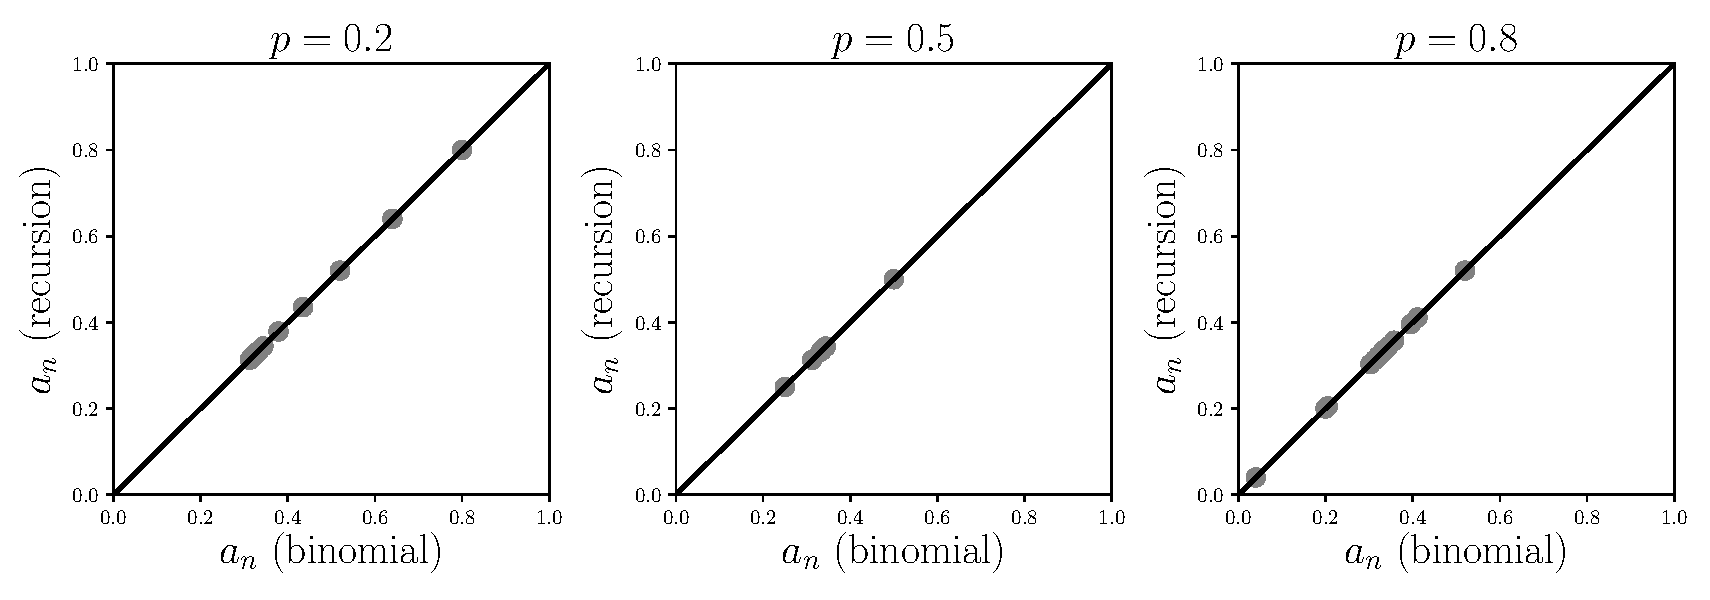
\includegraphics[totalheight=6cm]{chpt13/prob4.pdf}
  			  \caption{Comparison of $P(A_n)$ calculated recursively against $P(A_n)$ calculated with the binomial distribution (Problem 4).}
    			   \label{fig:prob_4}
	\end{figure}

\begin{lstlisting}
import numpy as np
from scipy.special import binom

def compute_binom_recur(p, N):
    """
    Compute probability that the number of heads out of N 
    coin flips (each of probability p) is divisible by 3.
    Returns the probability computed from the binomial
    distribution and the probability computed from recursion.
    """
    
    #compute the probability from the binomial
    P_arr=[]
    for n in range(1, N):
        P = np.sum(np.array([binom(n, 3*k)*p**(3*k)*(1-p)**(n-3*k)\
                             for k in range(0, int(np.floor(n/3)+1))]))
        P_arr.append(P)
     
    #compute the probability from recursion
    q = 1-p
    
    #initialize recursion
    an_HH = [0, 0, p]
    an_H = [0, 0, p**2]
    an = [q, q**2, p**3+q**3]
    
    for _ in range(N-4):
        #recursion update equations
        an_HH_new = an[-3]*p+an_HH[-1]*q
        an_H_new = an_HH_new*p+an_H[-1]*q
        an_new = an_H_new*p+an[-1]*q

        an_HH.append(an_HH_new)
        an_H.append(an_H_new)
        an.append(an_new)
        
    return (P_arr, an)
\end{lstlisting}
\end{problem}










